%%%%%%%%%%%%%%%%%%%%%%%%%%%%%%%%%%%%%%%%%%%%%%%%%%%%%%%%%%%%
%%  Class 2, NE 155
%%

\documentclass[xcolor=x11names,compress]{beamer}

\definecolor{CoolBlack}{rgb}{0.0, 0.18, 0.39}
%% General document %%%%%%%%%%%%%%%%%%%%%%%%%%%%%%%%%%
\usepackage{graphicx}
\usepackage{tikz}
\usetikzlibrary{decorations.fractals}
%%%%%%%%%%%%%%%%%%%%%%%%%%%%%%%%%%%%%%%%%%%%%%%%%%%%%%

%% Beamer Layout %%%%%%%%%%%%%%%%%%%%%%%%%%%%%%%%%%
\useoutertheme[subsection=false,shadow]{miniframes}
\useinnertheme{default}
\usefonttheme{serif}
\usepackage{palatino}
\usepackage{tabu}

% addition of color
\usepackage{xcolor}
\definecolor{dgreen}{rgb}{0.,0.6,0.}
\definecolor{RawSienna}{cmyk}{0,0.72,1,0.45}

\setbeamerfont{title like}{shape=\scshape}
\setbeamerfont{frametitle}{shape=\scshape}

\setbeamercolor*{lower separation line head}{bg=CoolBlack} 
\setbeamercolor*{normal text}{fg=black,bg=white} 
\setbeamercolor*{alerted text}{fg=red} 
\setbeamercolor*{example text}{fg=black} 
\setbeamercolor*{structure}{fg=black} 
 
\setbeamercolor*{palette tertiary}{fg=black,bg=black!10} 
\setbeamercolor*{palette quaternary}{fg=black,bg=black!10} 

\renewcommand{\(}{\begin{columns}}
\renewcommand{\)}{\end{columns}}
\newcommand{\<}[1]{\begin{column}{#1}}
\renewcommand{\>}{\end{column}}

% adding slide numbers
\addtobeamertemplate{navigation symbols}{}{%
    \usebeamerfont{footline}%
    \usebeamercolor[fg]{footline}%
    \hspace{1em}%
    \insertframenumber/\inserttotalframenumber
}

% equation stuff
\newcommand{\Macro}{\ensuremath{\Sigma}}
\newcommand{\Sn}{\ensuremath{S_N} }
\newcommand{\vOmega}{\ensuremath{\hat{\Omega}}}
\usepackage{mathrsfs}
\usepackage[mathcal]{euscript}
\usepackage{amssymb}
\usepackage{amsthm}
\usepackage{epsfig}
\usepackage{amsmath}
%%%%%%%%%%%%%%%%%%%%%%%%%%%%%%%%%%%%%%%%%%%%%%%%%%

\begin{document}

%%%%%%%%%%%%%%%%%%%%%%%%%%%%%%%%%%%%%%%%%%%%%%%%%%%%%%
%%%%%%%%%%%%%%%%%%%%%%%%%%%%%%%%%%%%%%%%%%%%%%%%%%%%%%
\begin{frame}
\title{NE 155\\Introduction to Numerical Simulations in Radiation Transport}
\subtitle{Lecture 2: Computers}
\author{
        Rachel Slaybaugh\\
        \vspace*{1em}
        {\it University of California, Berkeley\\
         Department of Nuclear Engineering}\\
}
\date{January 24, 2014}
\titlepage
\end{frame}

% Outline
% 1) History
%  - define flops as measure of what we care about
%  - chronological highlights of a few machines; show pictures, state details
%  - table of flops increasing number over years
% 2) Basic architecture
%  - hardware v software; we're talking about hardware now but the rest of the class will focus on software. We will care a little bit about the interface
%  - definitions
%  - Moore's law
% 3) Parallelism
%  - basic considerations
%  - types of parallelism
%  - speedup
%  - increase in use and potential
%  - current status
% 4) (if time; thw topic?) Discussion of parallelism architecture issues?
%  - Moore's law continuation?
%  - GPUs
%  - mic chips
%  - What happens may have a large impact on algorithms

%%%%%%%%%%%%%%%%%%%%%%%%%%%%%%%%%%%%%%%%%%%%%%%%%%%%%%
%%%%%%%%%%%%%%%%%%%%%%%%%%%%%%%%%%%%%%%%%%%%%%%%%%%%%%
\begin{frame}{Outline}
\begin{enumerate}
\item History and terminology
%  - define flops as measure of what we care about
%  - chronological highlights of a few machines; show pictures, state details
%  - table of flops increasing number over years
\item Basic computer architecture
%  - hardware v software; we're talking about hardware now but the rest of the class will focus on software. We will care a little bit about the interface
%  - definitions
%  - Moore's law
\item Introduction to Parallelism
%  - basic considerations
%  - types of parallelism
%  - speedup
%  - increase in use and potential
%  - current status
\item Current issues in hardware
%  - Moore's law continuation?
%  - GPUs
%  - mic chips
%  - What happens may have a large impact on algorithms
\end{enumerate}
\end{frame}

%%%%%%%%%%%%%%%%%%%%%%%%%%%%%%%%%%%%%%%%%%%%%%%%%%%%%%
%%%%%%%%%%%%%%%%%%%%%%%%%%%%%%%%%%%%%%%%%%%%%%%%%%%%%%
\section{History}
\begin{frame}{How do we measure utility?\footnote{en.wikipedia.org}}

\textbf{IPS} (Instructions Per Second) is a measure of a computer's processor speed. IPS can be useful when comparing performance between processors made from a similar architecture, but are difficult to compare between CPU architectures

\textbf{Clock rate} typically refers to the frequency at which a CPU is running. It is measured in the SI unit Hertz.

\textbf{FLOPS} (FLoating-point Operations Per Second) is a measure of computer performance, useful in fields of scientific calculations that make heavy use of floating-point calculations. 
\end{frame}

%%%%%%%%%%%%%%%%%%%%%%%%%%%%%%%%%%%%%%%%%%%%%%%%%%%%%%
%%%%%%%%%%%%%%%%%%%%%%%%%%%%%%%%%%%%%%%%%%%%%%%%%%%%%%
\begin{frame}{Computing Machines, Origins}

\begin{figure}
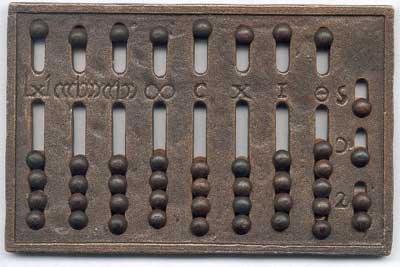
\includegraphics[height=2.25in,clip]{RomanAbacus}
\caption{Roman Abacus, http://history-computer.com/CalculatingTools/abacus.html}
\end{figure}

\end{frame}

%%%%%%%%%%%%%%%%%%%%%%%%%%%%%%%%%%%%%%%%%%%%%%%%%%%%%%
%%%%%%%%%%%%%%%%%%%%%%%%%%%%%%%%%%%%%%%%%%%%%%%%%%%%%%
\begin{frame}{Early Development of Computing}

\begin{figure}
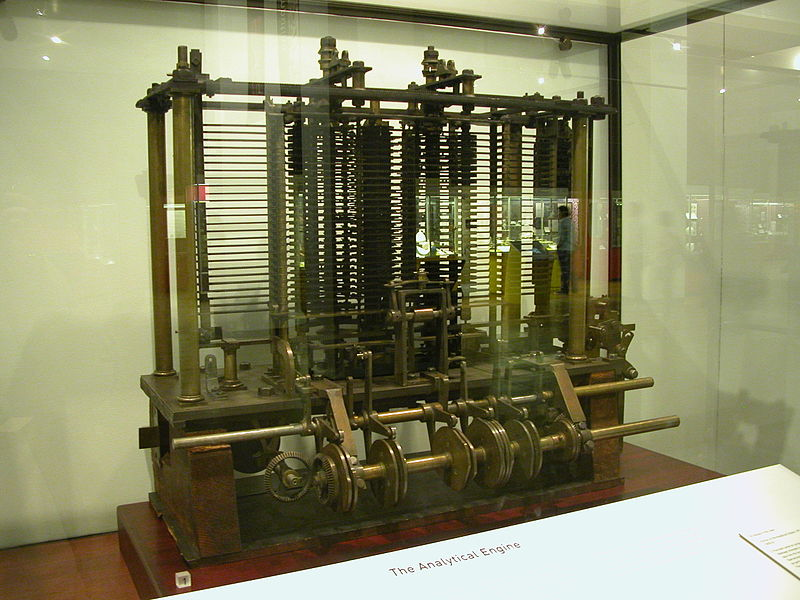
\includegraphics[height=2in,clip]{BabbageDiffMachine}
\caption{Reconstruction of Babbage's Analytical Engine, the first general-purpose programmable computer, http://en.wikipedia.org/wiki/History\_of\_computing\_hardware
\#Punched\_card\_data\_processing}
\end{figure}

\end{frame}

%%%%%%%%%%%%%%%%%%%%%%%%%%%%%%%%%%%%%%%%%%%%%%%%%%%%%%
%%%%%%%%%%%%%%%%%%%%%%%%%%%%%%%%%%%%%%%%%%%%%%%%%%%%%%
\begin{frame}{First Electromechanical Computers}

\begin{figure}
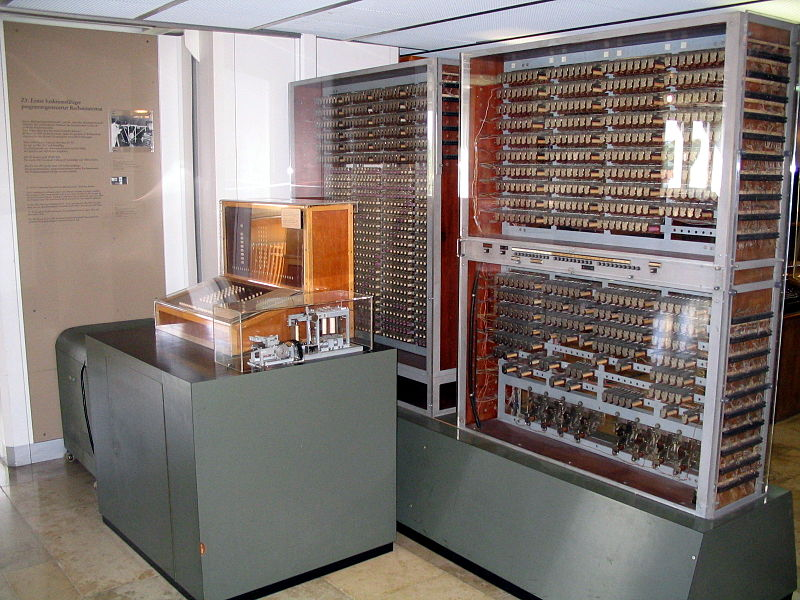
\includegraphics[height=2in,clip]{Z3DeutschesMuseum}
\caption{Zuse Z3 replica on display at Deutsches Museum in Munich, en.wikipedia.org/wiki/Z3\_(computer)}
\end{figure}

\end{frame}

%%%%%%%%%%%%%%%%%%%%%%%%%%%%%%%%%%%%%%%%%%%%%%%%%%%%%%
%%%%%%%%%%%%%%%%%%%%%%%%%%%%%%%%%%%%%%%%%%%%%%%%%%%%%%
\begin{frame}{Stored Programs}

\begin{figure}
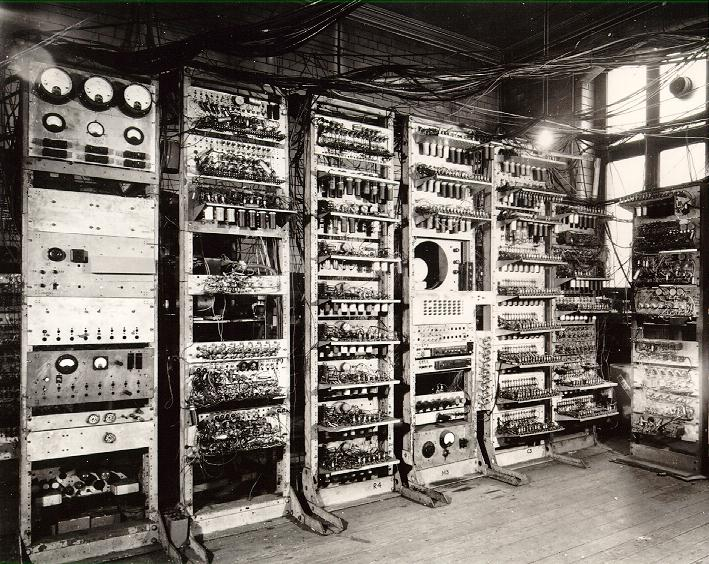
\includegraphics[height=2in,clip]{ManchesterMark1}
\caption{The Manchester Mark 1 was one of the world's first stored-program computers, http://www.computer50.org/mark1/ip-mm1.mark1.html}
\end{figure}

\end{frame}

%%%%%%%%%%%%%%%%%%%%%%%%%%%%%%%%%%%%%%%%%%%%%%%%%%%%%%
%%%%%%%%%%%%%%%%%%%%%%%%%%%%%%%%%%%%%%%%%%%%%%%%%%%%%%
\begin{frame}{Microprogramming, Magnetic Storage, Transistors}
\begin{itemize}
\item 1951: realization that CPUs can be controlled by a miniature, highly specialised computer program in high-speed ROM
\item 1954: magnetic core memory was rapidly displacing most other forms of temporary storage
\item 1956: IBM introduced the first disk storage unit: using 50 24-inch metal disks, it stored 5 MB of data for \$10,000 per MB (\$90,000 in 2014 \$s)
\item 1947: invention of the bipolar transistor; this replaced vacuum tubes by 1955 $\rightarrow$ ``Second Generation" of computer designs
\end{itemize}
\end{frame}

%%%%%%%%%%%%%%%%%%%%%%%%%%%%%%%%%%%%%%%%%%%%%%%%%%%%%%
%%%%%%%%%%%%%%%%%%%%%%%%%%%%%%%%%%%%%%%%%%%%%%%%%%%%%%
\begin{frame}{Supercomputers}

\begin{figure}
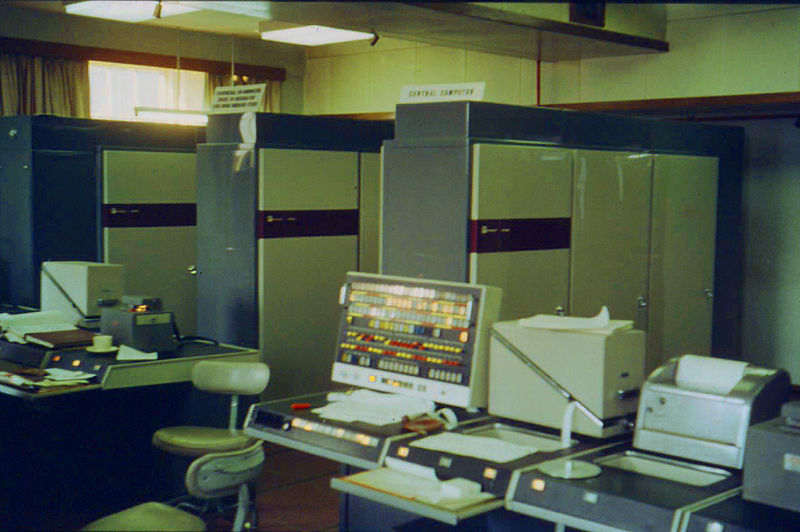
\includegraphics[height=2in,clip]{Atlas1963}
\caption{The University of Manchester Atlas 1963, http://en.wikipedia.org/wiki/History\_of\_computing\_hardware
\#Punched\_card\_data\_processing}
\end{figure}

\end{frame}

%%%%%%%%%%%%%%%%%%%%%%%%%%%%%%%%%%%%%%%%%%%%%%%%%%%%%%
%%%%%%%%%%%%%%%%%%%%%%%%%%%%%%%%%%%%%%%%%%%%%%%%%%%%%%
\begin{frame}{Integrated Circuit}
With the advent of the transistor and the work on semi-conductors generally, it now seems possible to envisage electronic equipment in a solid block with no connecting wires. The block may consist of layers of insulating, conducting, rectifying and amplifying materials, the electronic functions being connected directly by cutting out areas of the various layers.\\
\vspace*{1.5 em}
\hspace*{0.5 in}Geoffrey W.A. Dummer, Royal Radar Establishment of the Ministry of Defence, 1952

\end{frame}

%%%%%%%%%%%%%%%%%%%%%%%%%%%%%%%%%%%%%%%%%%%%%%%%%%%%%%
%%%%%%%%%%%%%%%%%%%%%%%%%%%%%%%%%%%%%%%%%%%%%%%%%%%%%%
\begin{frame}{Generations 4-6}
\begin{itemize}
\item Very large scale integration of devices on chip
\item C and FORTRAN programming languages
\item UNIX operating system (Bell labs, Berkeley)
\item Large scale parallel processing; supercomputing centers
\item Shared and distributed memory
\item Parallel/vector shared/distributed memory combinations
\item High speed networking
\end{itemize}
\end{frame}

%%%%%%%%%%%%%%%%%%%%%%%%%%%%%%%%%%%%%%%%%%%%%%%%%%%%%%
%%%%%%%%%%%%%%%%%%%%%%%%%%%%%%%%%%%%%%%%%%%%%%%%%%%%%%
\begin{frame}{Easy?}
 \begin{figure}
   \begin{center}
     %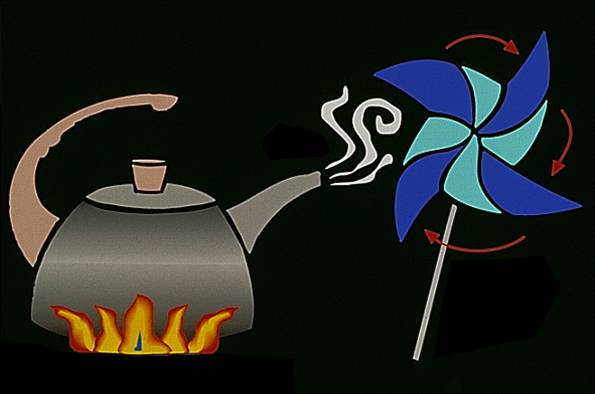
\includegraphics[height=2.5in,clip]{TeaPot}
   \end{center}
 \end{figure}
\end{frame}

%%%%%%%%%%%%%%%%%%%%%%%%%%%%%%%%%%%%%%%%%%%%%%%%%%%%%%
%%%%%%%%%%%%%%%%%%%%%%%%%%%%%%%%%%%%%%%%%%%%%%%%%%%%%%
\begin{frame}{What are we trying to accomplish?}
\begin{itemize}
\item In order to design economical and safe reactors, one must choose among a vast range of competing designs:
\begin{itemize}
\item What are the best fuels, structure, and coolant materials; what are their appropriate ratios?
\item How does the reactor respond to component failures?
\item How does one balance those choices given competing goals of performance, lifetime, safety, and capital cost?
\end{itemize}
\item Ideally, one would like to base these choices on theory rather than experimental trial and error.
\item This is where \textcolor{dgreen}{computational science} fits in...
\end{itemize}
\end{frame}

%%%%%%%%%%%%%%%%%%%%%%%%%%%%%%%%%%%%%%%%%%%%%%%%%%%%%%
%%%%%%%%%%%%%%%%%%%%%%%%%%%%%%%%%%%%%%%%%%%%%%%%%%%%%%
\begin{frame}{Early Days}
Before much computer use (e.g., 1943), things took a long time
\begin{tabu}{|X | l|}
\hline
Project & Est. Time \\\hline
Density distribution in difficult system & 2 weeks \\
Integral equation for absorption in Al slab & 2 weeks \\
Slowing-down length in H$_2$O \& related calcs & 3 weeks \\
Albedo problems & 1 week \\\hline
\end{tabu}
\begin{center}
%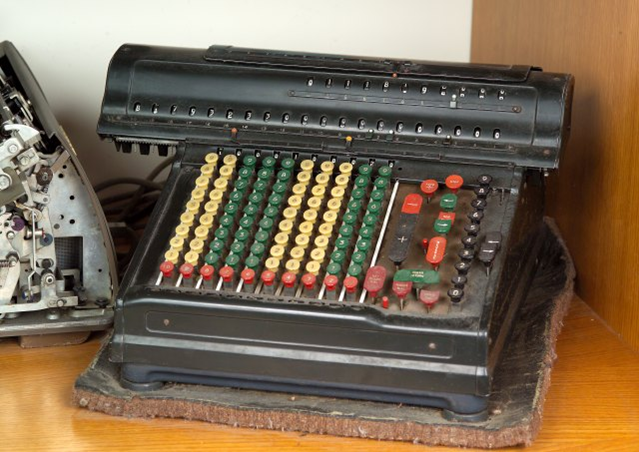
\includegraphics[height=1.5in,clip]{ACRM}
\end{center}
\end{frame}

%%%%%%%%%%%%%%%%%%%%%%%%%%%%%%%%%%%%%%%%%%%%%%%%%%%%%%
%%%%%%%%%%%%%%%%%%%%%%%%%%%%%%%%%%%%%%%%%%%%%%%%%%%%%%
\begin{frame}{Adolescence -- Early 1980s}
\begin{itemize}
\item NE was at the forefront of computer applications (!)
%pushing the envelope for ever greater computing resources and related advances in computational science.
\item Major early success story in the computational sciences:
\begin{itemize}
\item Reduced the burden of experiment
\item Contributed greatly to reactor design
\end{itemize}
\item However, modeling was severely constrained 
%Even state-of-the-art machines such as Cray-1 were 
\begin{itemize}
\item Unable to explicitly model the key physical phenomena within a reactor
\item Low-dimensional representation
\item Lumped parameter models
\item Empirical correlations with tunable parameters established largely by experiments
\end{itemize}
\end{itemize}
\end{frame}

%%%%%%%%%%%%%%%%%%%%%%%%%%%%%%%%%%%%%%%%%%%%%%%%%%%%%%
%%%%%%%%%%%%%%%%%%%%%%%%%%%%%%%%%%%%%%%%%%%%%%%%%%%%%%
\begin{frame}{Adolescence $\rightarrow$ Today's Challenges}
\begin{itemize}
\item Computing limitations caused
\begin{itemize}
\item Heavy reliance on expensive and often complicated experiments
\item Inaccuracy resulted in \emph{significant design margins} $\rightarrow$ negative impact on plant economics
\item Exploration of novel reactor design concepts was greatly constrained 
%by fundamental limitations in the predictability of the models
\end{itemize}
\item Many codes developed then are still used 
\item Can we update these tools?
\item Do we need to design new tools?
\item What methods will take us into the future?
\item What will the architectures look like?
\item How do we successfully navigate that interplay?
\end{itemize}
\end{frame}

%%%%%%%%%%%%%%%%%%%%%%%%%%%%%%%%%%%%%%%%%%%%%%%%%%%%%%
%%%%%%%%%%%%%%%%%%%%%%%%%%%%%%%%%%%%%%%%%%%%%%%%%%%%%%
\begin{frame}{Current State}
2010: the DOE announced \emph{Oak Ridge National Laboratory} won the Nuclear Energy Modeling and Simulation Energy Innovation Hub (\$122 million for 5 years), including:	
\begin{itemize}
\item Electric Power Research Institute (EPRI), Palo Alto, CA
\item Idaho National Laboratory, Idaho Falls, ID
\item Los Alamos National Laboratory, Los Alamos, NM
\item Massachusetts Institute of Technology, Cambridge, MA
\item North Carolina State University, Raleigh, NC
\item Sandia National Laboratories, Albuquerque, NM
\item Tennessee Valley Authority, Knoxville, TN
\item University of Michigan, Ann Arbor, MI
\item Westinghouse Electric Company, Pittsburgh, PA
\end{itemize}
\end{frame}

%%%%%%%%%%%%%%%%%%%%%%%%%%%%%%%%%%%%%%%%%%%%%%%%%%%%%%
%%%%%%%%%%%%%%%%%%%%%%%%%%%%%%%%%%%%%%%%%%%%%%%%%%%%%%
\begin{frame}{Consortium for Advanced Simulation of Light Water Reactors}
\begin{center}
%
\includegraphics[height=0.75in,clip]{CASL}
\end{center}
\begin{itemize}
\item \textcolor{RawSienna}{TASK 1}: develop computer models that simulate nuclear power plant operations, forming a ``virtual reactor" for the predictive simulations of light water reactors. 
\item \textcolor{RawSienna}{TASK 2}: use computer models to reduce capital and operating costs per unit of energy, extend the lifetime of the existing U.S. reactor fleet, and reduce nuclear waste volume generated by enabling higher fuel burn-ups... %\\The CASL virtual reactor will also be used to accelerate the deployment of next-generation reactor designs, particularly advanced nuclear fuel technologies and structural materials within the reactor core.
\end{itemize}
\end{frame}

%%%%%%%%%%%%%%%%%%%%%%%%%%%%%%%%%%%%%%%%%%%%%%%%%%%%%%
%%%%%%%%%%%%%%%%%%%%%%%%%%%%%%%%%%%%%%%%%%%%%%%%%%%%%%
\begin{frame}{Supercomputing in Research}
These kinds of simulations require time on the fastest computers in the world
\begin{itemize}
\item \textcolor{RawSienna}{Titan} (ORNL): 299,008 Opteron Cores (CPU) + 18,688 K21 Keplers (GPU); 27 petaflops 
\item \textcolor{RawSienna}{IBM Sequoia} (LLNL): 1,572,864 cores (CPU); \\16.32 petaflops
\end{itemize}
\begin{figure}
%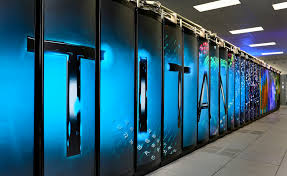
\includegraphics[height=1.1in,clip]{Titan}
\hfill
%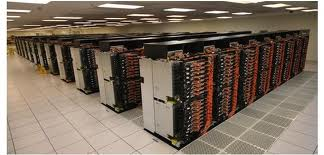
\includegraphics[height=1.1in,clip]{Sequoia}
\end{figure}
\end{frame}

%%%%%%%%%%%%%%%%%%%%%%%%%%%%%%%%%%%%%%%%%%%%%%%%%%%%%%
%%%%%%%%%%%%%%%%%%%%%%%%%%%%%%%%%%%%%%%%%%%%%%%%%%%%%%
\begin{frame}{It's Important}
``. . . At Oak Ridge National Laboratory, they're using supercomputers to get a lot more power out of our nuclear facilities . . . . "

\vspace*{0.5 in}
President Obama, 2011 State of the Union\\
http://www.casl.gov/media/20110127\_news.shtml
\end{frame}

%%%%%%%%%%%%%%%%%%%%%%%%%%%%%%%%%%%%%%%%%%%%%%%%%%%%%%
%%%%%%%%%%%%%%%%%%%%%%%%%%%%%%%%%%%%%%%%%%%%%%%%%%%%%%
\begin{frame}{What Can We Accomplish?}
\begin{itemize}
\item Predictive simulation 
\item Model entire facilities at a new level of fidelity
\item Coupled multi-physics
%Lets us reduce margins, extend existing reactor lifetimes, and consider new designs.
\end{itemize}
\begin{figure}
%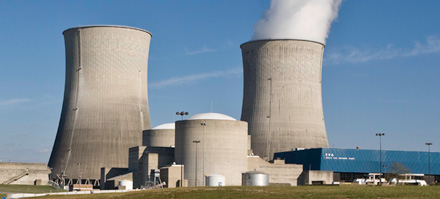
\includegraphics[height=1.2in,clip]{WattsBar}
\hfill
%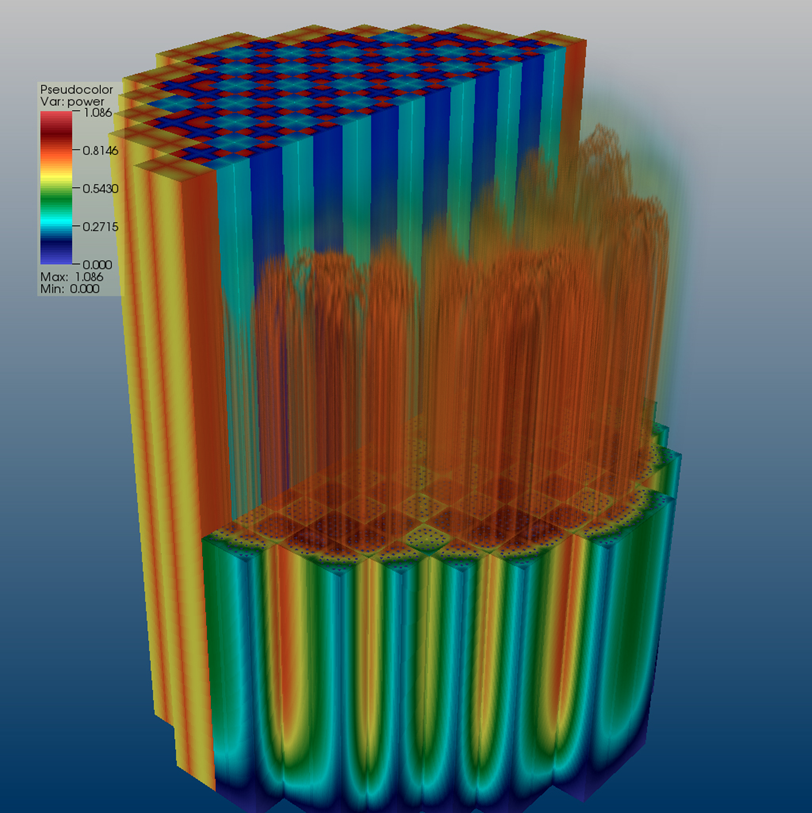
\includegraphics[height=1.2in,clip]{DenovoCore}
\end{figure}
\end{frame}

%%%%%%%%%%%%%%%%%%%%%%%%%%%%%%%%%%%%%%%%%%%%%%%%%%%%%%
%%%%%%%%%%%%%%%%%%%%%%%%%%%%%%%%%%%%%%%%%%%%%%%%%%%%%%
\begin{frame}{What Can We Accomplish?}
\underline{Integrate}
\begin{itemize}
\item existing nuclear energy and nuclear national security modeling and simulation capabilities
\item and associated expertise
\item with high-performance computing
\end{itemize}    
to solve problems that were \emph{previously unthinkable or impractical} in terms of the computing power required to address them

\vspace*{1em}
However, these computer simulations will not completely eliminate the need for \emph{experimental or measurement data} to confirm or ``validate" the software. 

\vspace*{1em}
\hspace*{0.25 in} John Wagner, ORNL
\end{frame}

%"Traditionally, reactor models for radiation dose assessments have considered just the reactor core, or a small part of the core," Wagner says. "However, we're now simulating entire nuclear facilities, such as a nuclear power reactor facility with its auxiliary buildings and the ITER fusion reactor, with much greater accuracy than any other organization that we're aware of." 
%
%More accurate models enable nuclear plants to be designed with more accurate safety margins and shielding requirements, which helps to improve safety and reduce costs. The technology that makes this sort of leading-edge simulation possible is a combination of ORNL's Jaguar, the world's fastest supercomputer; advanced transport methods; and a next-generation software package called Denovo.
%
%DENOVO is a Scalable HPC Transport Code for Multi-Scale Nuclear Energy Applications
%http://computing.ornl.gov/SC09/videos/tomevans_1Mb.mov

%%%%%%%%%%%%%%%%%%%%%%%%%%%%%%%%%%%%%%%%%%%%%%%%%%%%%%
%%%%%%%%%%%%%%%%%%%%%%%%%%%%%%%%%%%%%%%%%%%%%%%%%%%%%%
\begin{frame}{Questions?}
\begin{figure}
%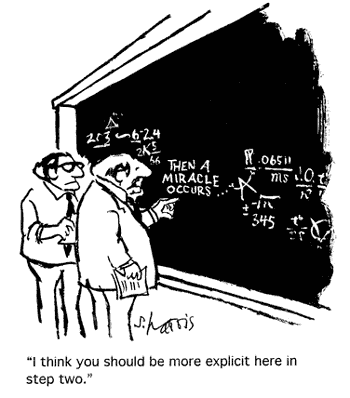
\includegraphics[height=3in,clip]{math07}
\end{figure}
\end{frame}

\end{document}